\subsection{Comparison of Solver Performance}

The computational performance of the four numerical methods
was compared using the selected pseudo-time steps:
$\Delta t=0.265$ for AFI, $\Delta t=1$ for the direct
implicit solver, $\Delta t=0.017$ for RK2, and
$\Delta t=0.024$ for RK4. These values were selected based
on the preceding time-step and stability analyses. The
explicit methods use time steps slightly below their
estimated stability limits, while the direct solver uses
a representative time step of $1$ rather than an
excessively large value.

All simulations were performed on the same $50\times20$
grid with $\mathrm{Pe}=17.5$, $\mathrm{Br}=0.2$, and a
convection coefficient of $1$. Five independent runs
were performed for each method, with the initial
temperature field reconstructed before every run. The
convergence criterion was a steady-state residual
tolerance of $10^{-12}$. The elapsed wall-clock time was
measured around each solver call, including solver-specific
setup operations such as matrix assembly and factorization.
The construction of the initial temperature and velocity
fields and the independent residual evaluation were
excluded from the measured time.

Table~\ref{tab:solver_comparison} summarizes the results.
All five runs of each method converged to the prescribed
residual tolerance. The reported computation times are
the medians of the five runs, and the standard deviations
indicate the variation in runtime.

\begin{table}[htbp]
    \centering
    \small
    \caption{Performance comparison of the four numerical
    methods on the $50\times20$ grid.}
    \label{tab:solver_comparison}
    \begin{tabular}{@{}l c c c c c@{}}
        \hline
        Method
        & $\Delta t$
        & Iterations
        & Median time (s)
        & Std. dev. (s)
        & Final residual
        \\
        \hline
        AFI
        & $0.265$
        & $295$
        & $6.2817$
        & $0.1800$
        & $9.398\times10^{-13}$
        \\[0.1cm]
        Direct implicit Euler
        & $1.0$
        & $16$
        & $0.1403$
        & $0.0094$
        & $6.322\times10^{-13}$
        \\[0.1cm]
        Explicit RK2
        & $0.017$
        & $392$
        & $8.0148$
        & $0.1089$
        & $9.907\times10^{-13}$
        \\[0.1cm]
        Explicit RK4
        & $0.024$
        & $309$
        & $10.7187$
        & $0.1100$
        & $9.748\times10^{-13}$
        \\
        \hline
    \end{tabular}
\end{table}

In addition to the final performance measurements, the
convergence histories were examined to compare the
behavior of the methods throughout the iterations.
Figures~\ref{fig:residual_vs_iteration} and
\ref{fig:residual_vs_time} show the steady-state residual
as a function of iteration number and elapsed computation
time, respectively. For each method, the plotted history
corresponds to the successful run whose total runtime was
closest to the median runtime of its five runs. This
provides a representative convergence history for each
method without superimposing all five runs.

\begin{figure}[htbp]
    \centering
    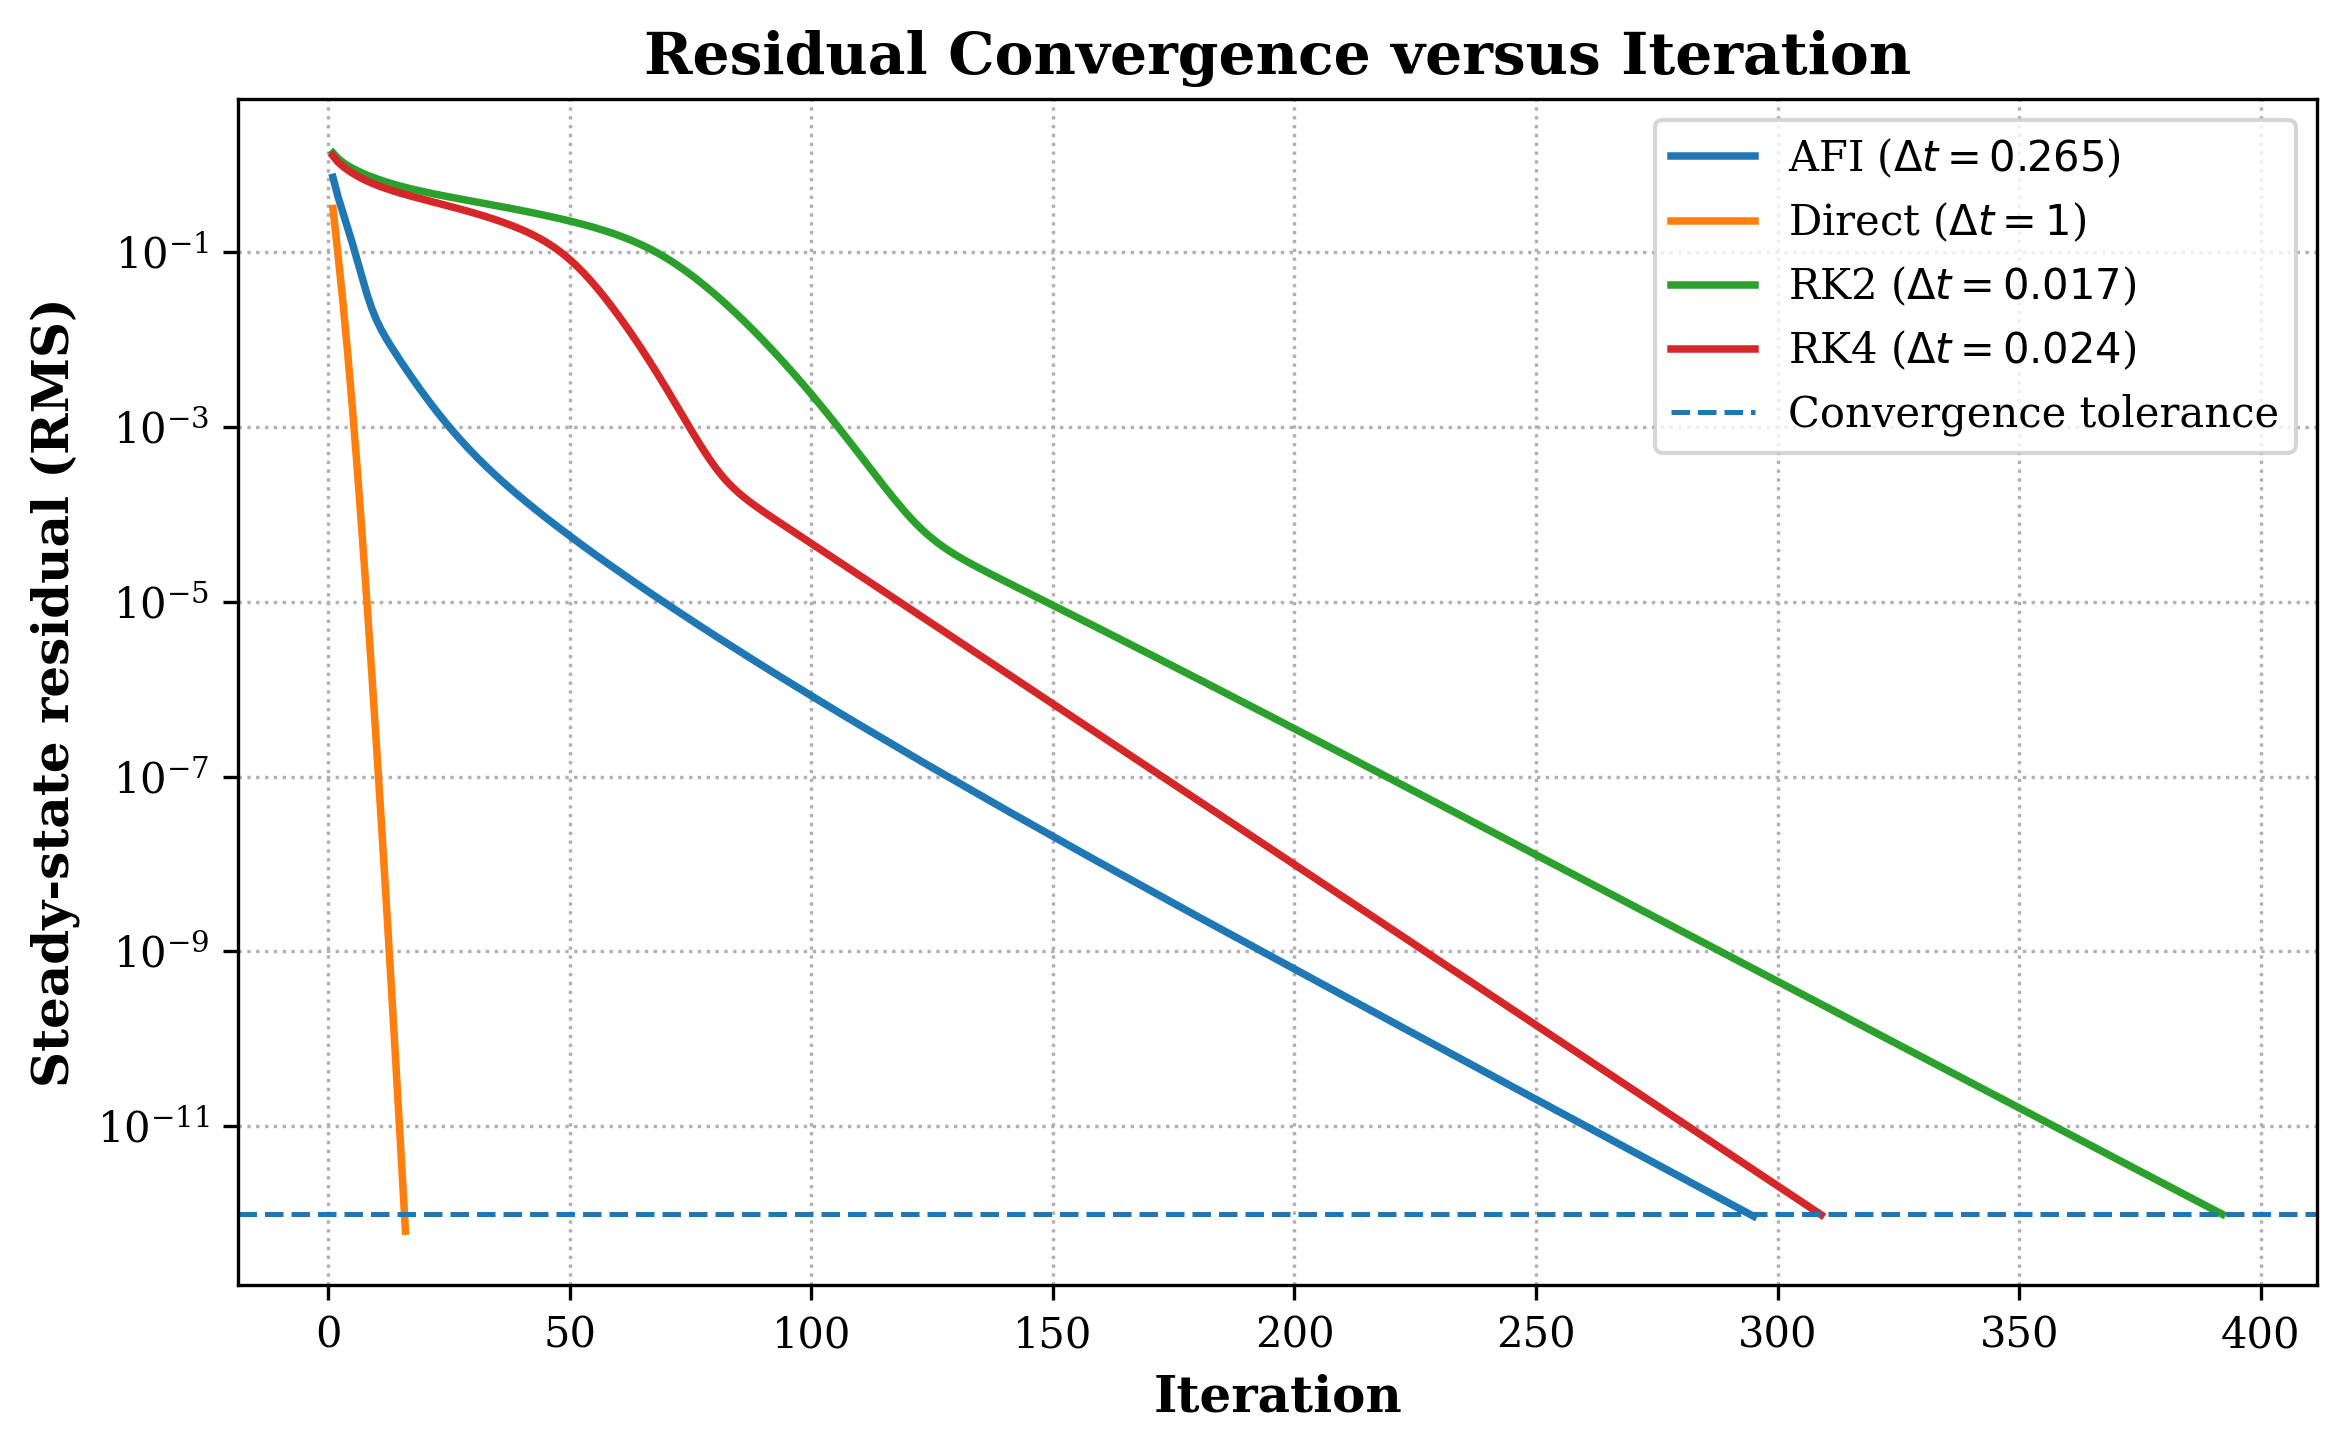
\includegraphics[width=0.85\textwidth]
    {figures/residual_vs_iteration.png}
    \caption{Steady-state residual versus iteration number
    for the four numerical methods. The dashed line
    indicates the convergence tolerance of $10^{-12}$.}
    \label{fig:residual_vs_iteration}
\end{figure}

Figure~\ref{fig:residual_vs_iteration} compares the
convergence behavior in terms of iteration count. The
direct implicit solver reached the prescribed tolerance
in only 16 iterations, compared with 295 for AFI, 392
for RK2, and 309 for RK4. RK4 required fewer iterations
than RK2, while the direct method converged in
substantially fewer iterations than the other methods.

\begin{figure}[htbp]
    \centering
    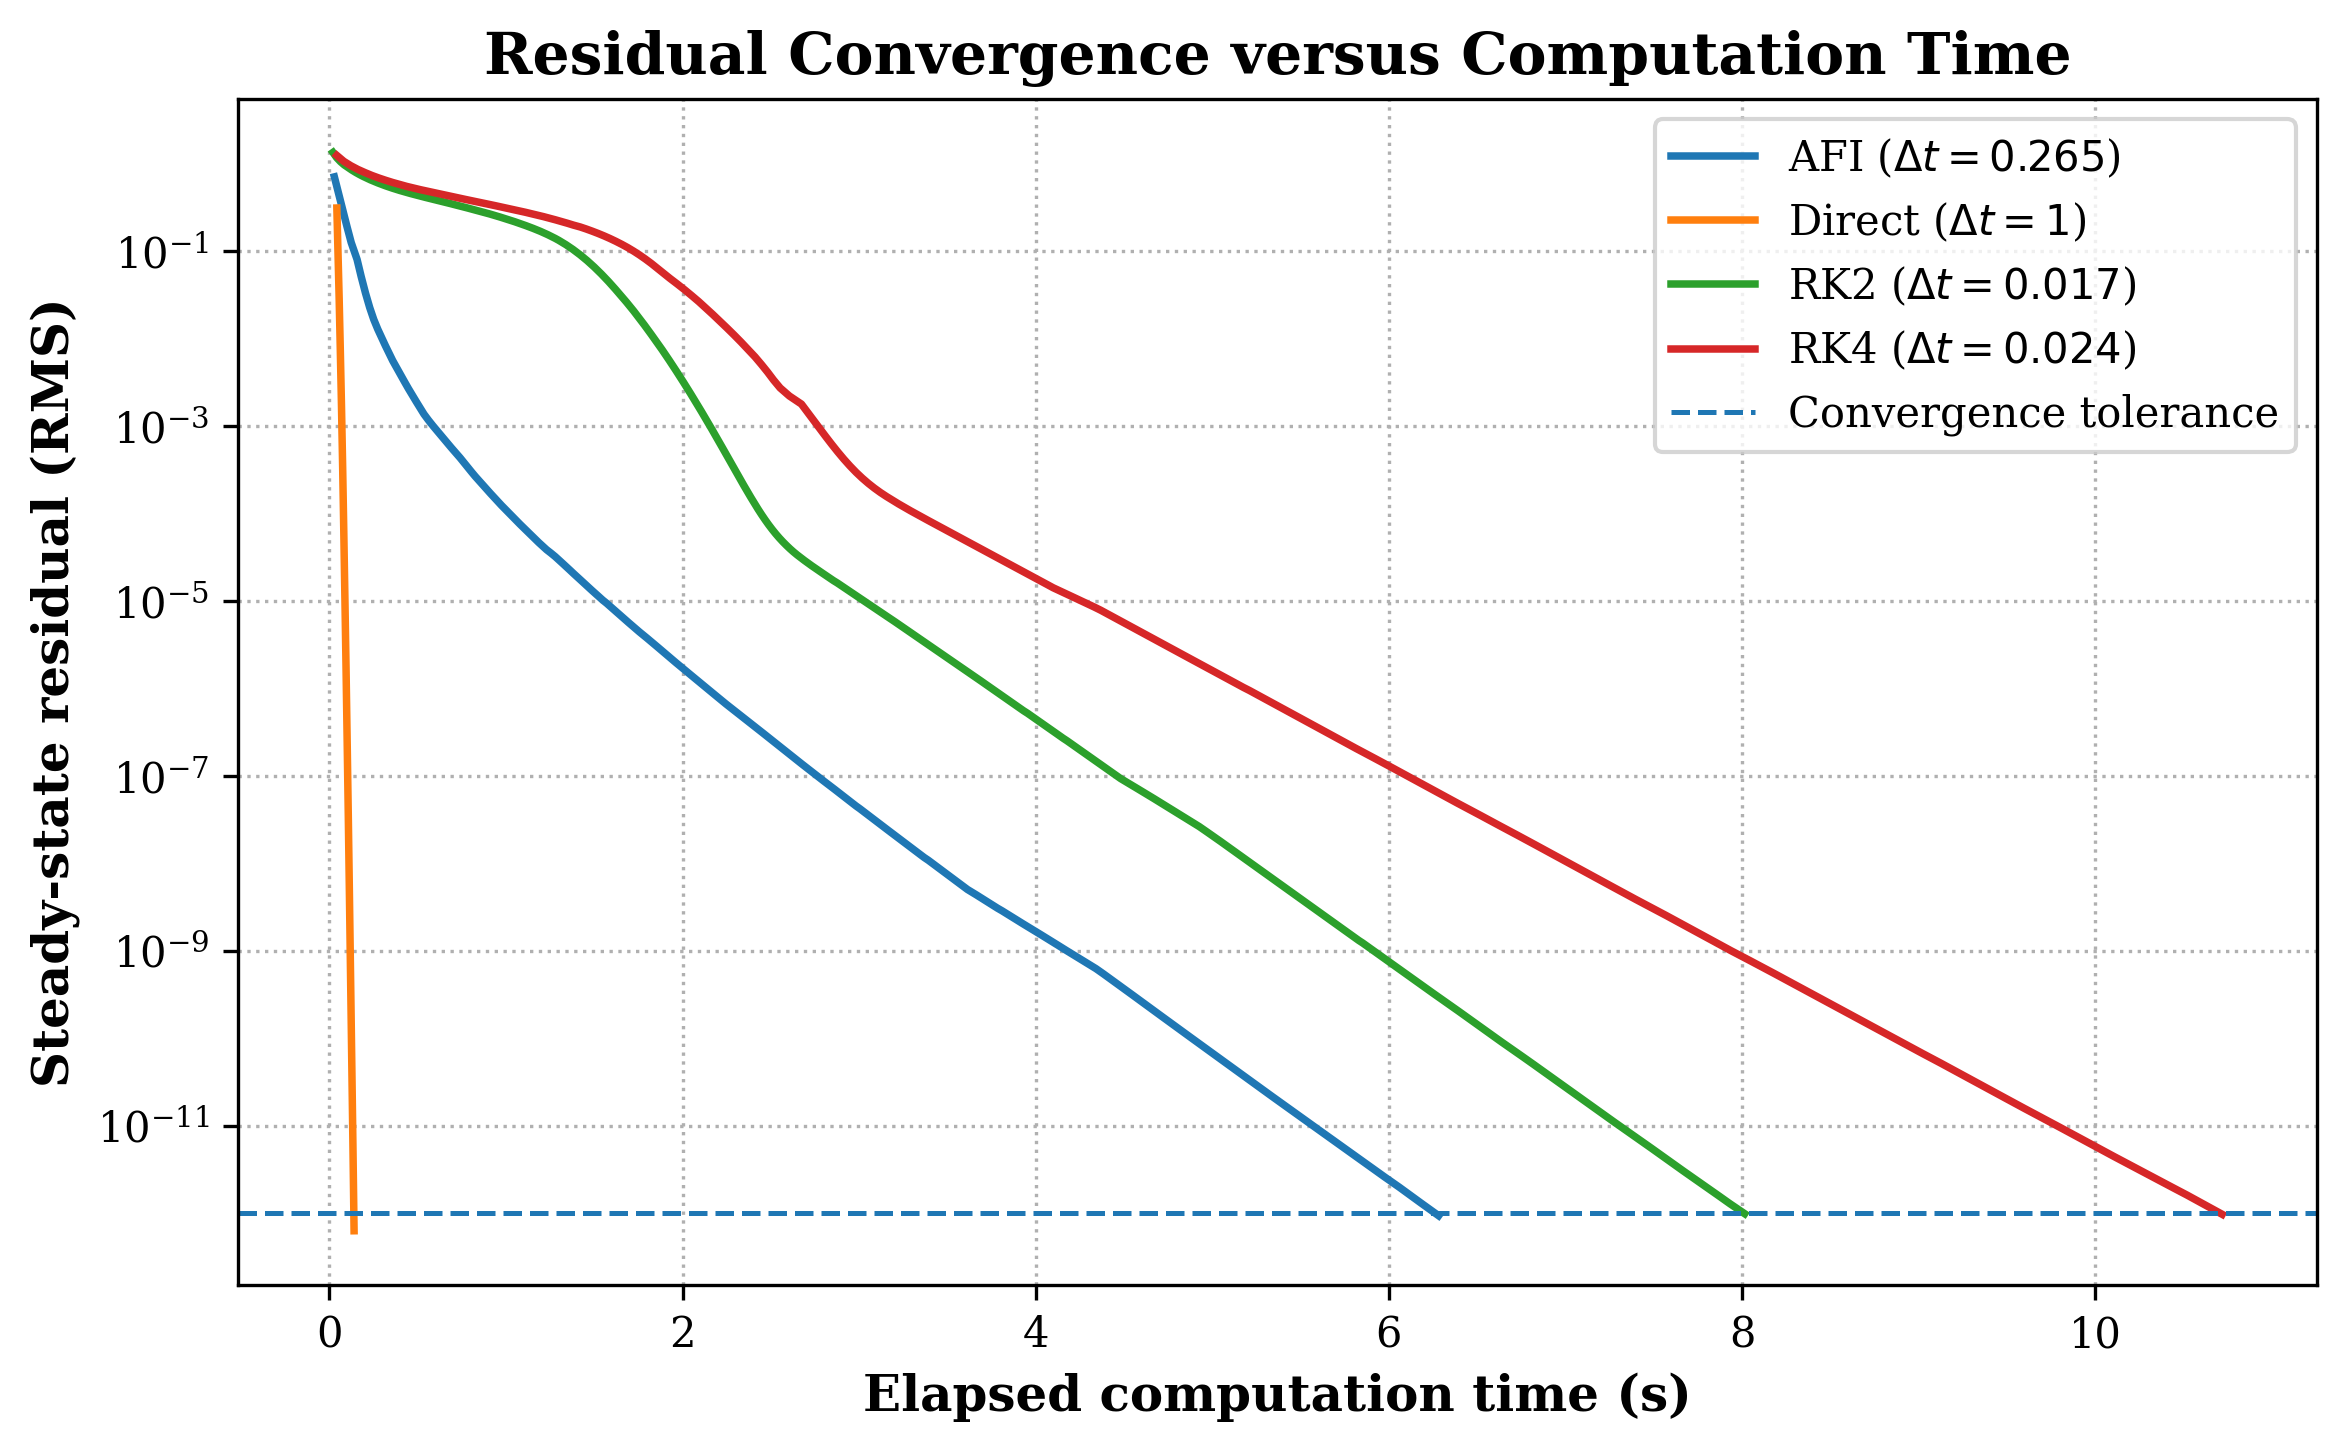
\includegraphics[width=0.85\textwidth]
    {figures/residual_vs_time.png}
    \caption{Steady-state residual versus elapsed
    computation time for the four numerical methods.
    The dashed line indicates the convergence tolerance
    of $10^{-12}$.}
    \label{fig:residual_vs_time}
\end{figure}

The residual-versus-time histories provide a direct
comparison of the computational effort required to
reach the prescribed convergence tolerance. The direct
implicit solver achieved the lowest median computation
time, at $0.1403~\mathrm{s}$. Relative to this method,
AFI, RK2, and RK4 required approximately 44.8, 57.1,
and 76.4 times more computation time, respectively.
Although RK4 required fewer iterations than RK2, its
overall computation time was higher. This is consistent
with the greater computational cost of its four-stage
time-integration procedure compared with the two-stage
RK2 method.

AFI was faster than both explicit Runge--Kutta methods
for the selected time steps, despite requiring more
iterations than RK4 and fewer than RK2. This indicates
that iteration count alone does not determine the
computational cost; the operations required within each
iteration also influence the total runtime.

All four methods satisfied the same steady-state
residual criterion in all five runs. The direct implicit
solver was the most computationally efficient among
the tested methods. However, these runtime ratios apply
specifically to the present grid, implementation, and
selected time steps. They should not be interpreted as
general performance rankings for other grid sizes or
problem configurations.
